\documentclass{article}

\usepackage{graphicx}
\usepackage{amsmath}
\usepackage{mathtools}
\usepackage[utf8]{inputenc}
\usepackage{framed}
\usepackage[T1]{fontenc}
\usepackage{listings}
\usepackage{amssymb}
\usepackage{verbatim}
\usepackage{array}
\usepackage{nth}
\usepackage{csvsimple}
\usepackage{tabularx}
\usepackage{wrapfig}

\setlength\parindent{0pt} % Removes all indentation from paragraphs
\usepackage[left=3cm,top=2cm,right=3cm,nohead,nofoot]{geometry}



\title{Project Proposal: Trafic Lights Controller}

\author{Jamal \textsc{Ben Azouze}, Marien \textsc{Bourguignon},\\ Nicolas \textsc{De Groote}, Simon \textsc{Picard}, Arnaud \textsc{Rosette}} % Author name

\date{\today} % Date for the report

\begin{document}

\maketitle % Insert the title, author and date


\section{Introduction}
\subsection{Basic idea of our project}
\begin{wrapfigure}{r}{0.2\textwidth}
  \begin{center}
    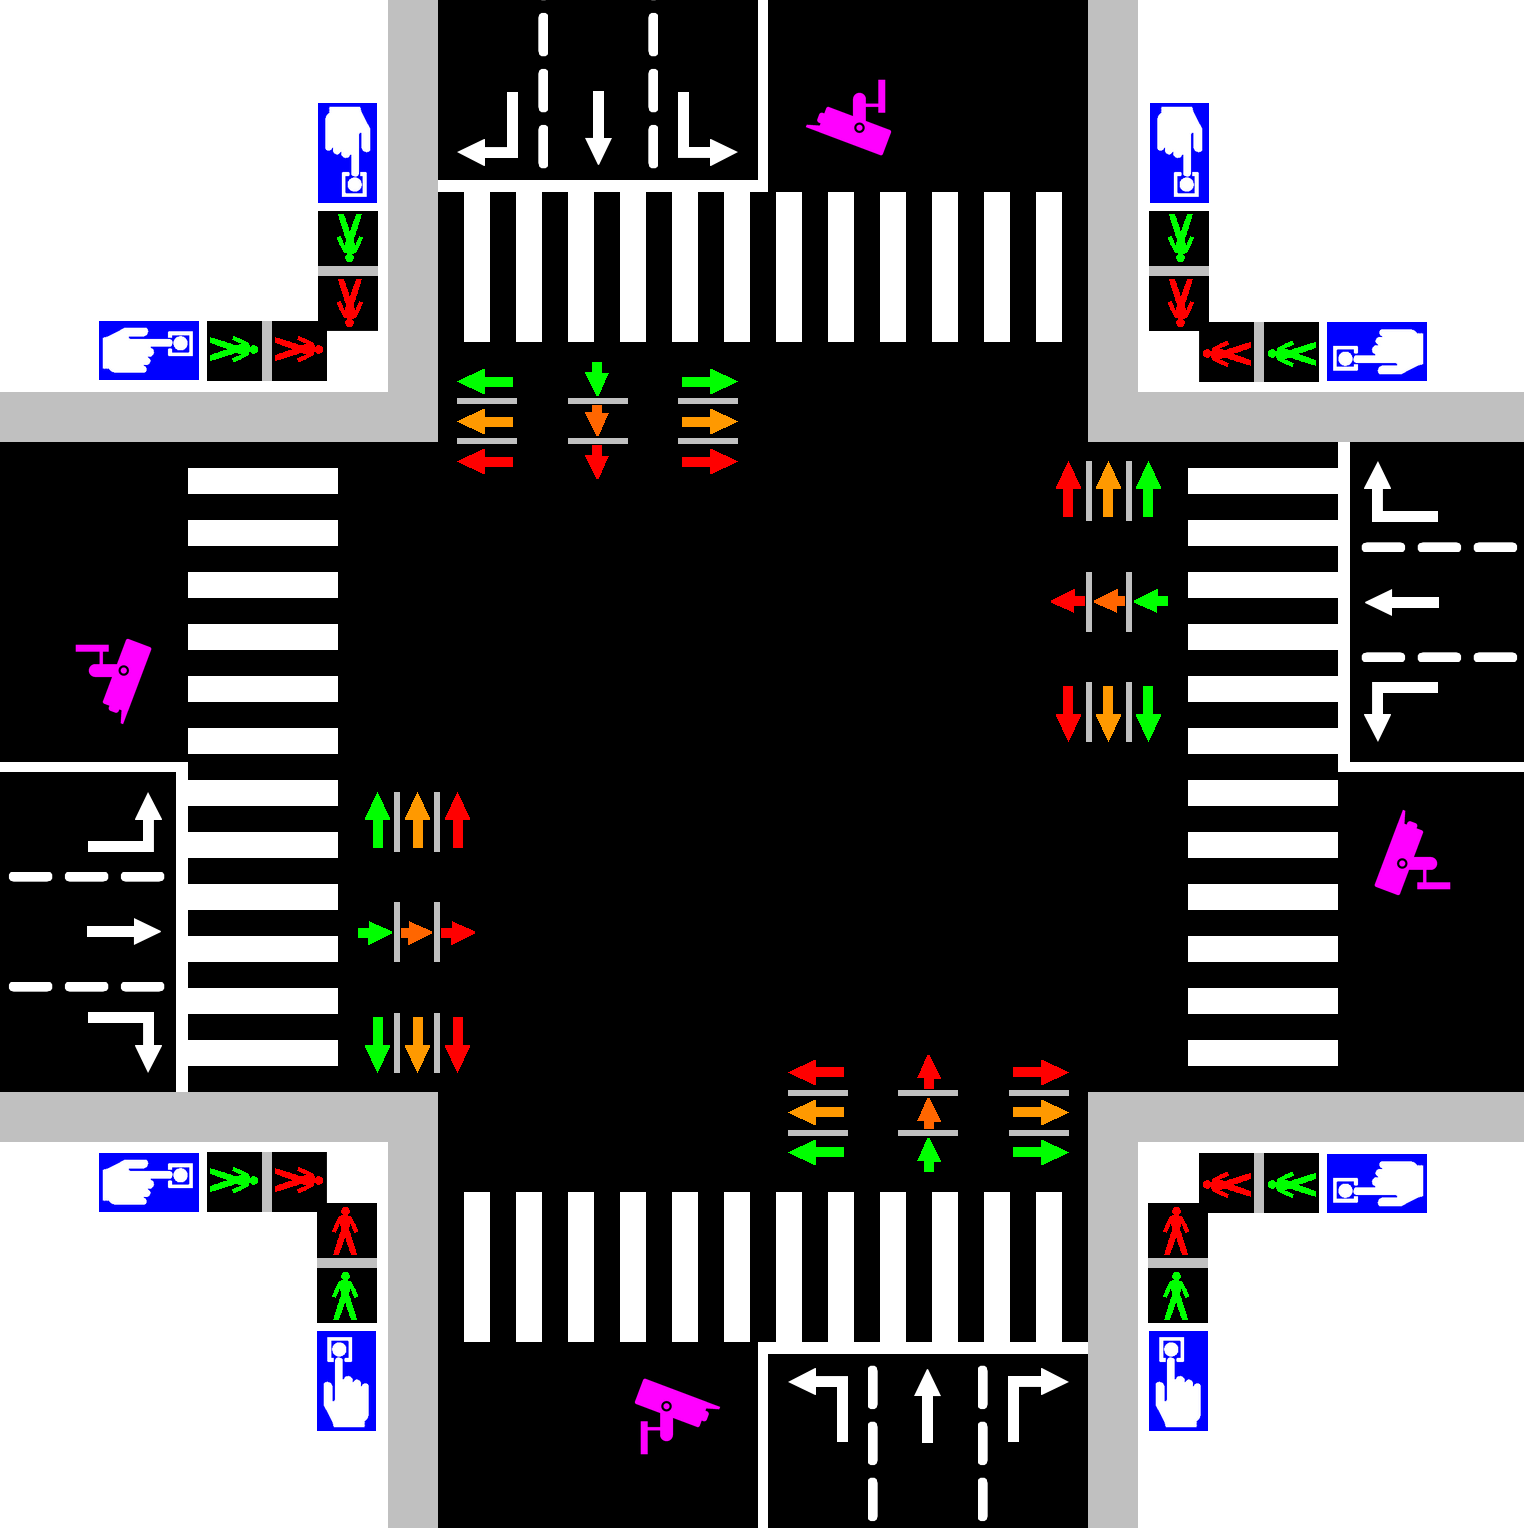
\includegraphics[width=0.25\textwidth]{schema.png}
  \end{center}
\end{wrapfigure}
\paragraph{}
The goal of our project is to design a controller for trafic lights at a crossing junction. The system will have push buttons for pedestrians to notify that they want to cross.
There will also be detectors to inform the controller on how many cars are waiting at the red lights to assign some kind of priorities, while still taking into account the pedestrians.

\paragraph{}
Because we are a group of 6, we choosed to work on a four-way instead of a simple junction. As we can see on the right, we have four crosswalks and two pairs of traffic lights to orchestrate. The pink cameras represent car detectors. Ultimately, we should come up with a solution to avoid unwanted situations which are explained below.

\paragraph{}
To be noted that we do the project conjointly with the course of embedded system.\\ 



\subsection{Why using model checking?}
\paragraph{}
In such a system, lives are at stake. If the lights get mixed up, we could easily reach a state where pedestrians and cars cross the road at the same time, or even in a situation where head-on collision could happen. This is why it is important to formally check our model and remove the chances of reaching problematic states.
\paragraph{}
Another interesting reason as of why our project could benefit from model checking is the real-time dimension. Indeed, a clogged junction increases the risk of accident (and also affects people's moods). Designing a controller to allow a fluid circulation could make commuting safer.


\end{document}
